\documentclass{beamer}
\setbeamertemplate{mini frames}{}
\usepackage{xcolor}
\usepackage{amsthm}
\usepackage{lipsum}
\usepackage{hyperref}
\usepackage[magyar]{babel}
\usepackage{t1enc}
\usetheme{Warsaw}
\usecolortheme{rose}
\frenchspacing
\usepackage{wrapfig}



\title{Videókártyák}
\author{Buha Milán, \\Kórád György}
\date{2022}

\begin{document}
\frame{\titlepage}
\frame{\tableofcontents}

\section{Bevezetés}
\begin{frame}
\frametitle{Bevezetés}
\framesubtitle{Mi az a videókártya?}
Feladata, hogy a számítógép által küldött képi információkat feldolgozza, és egy megjelenítő egység számára értelmezhető analóg jelekké alakítsa. Ez az egység monitor, TV vagy kivetítő is lehet. A grafikus kártya és a megjelenítő különböző grafikus szabványok szerint kommunikálhat egymással. A videókártya a kivitelezés alapján lehet alaplapra integrált vagy bővítőkártya.
\end{frame}

\subsection{Története}
\begin{frame}
\frametitle{Bevezetés}
\framesubtitle{Története}
\begin{wrapfigure}{r}{0.3\textwidth}
    \centering
    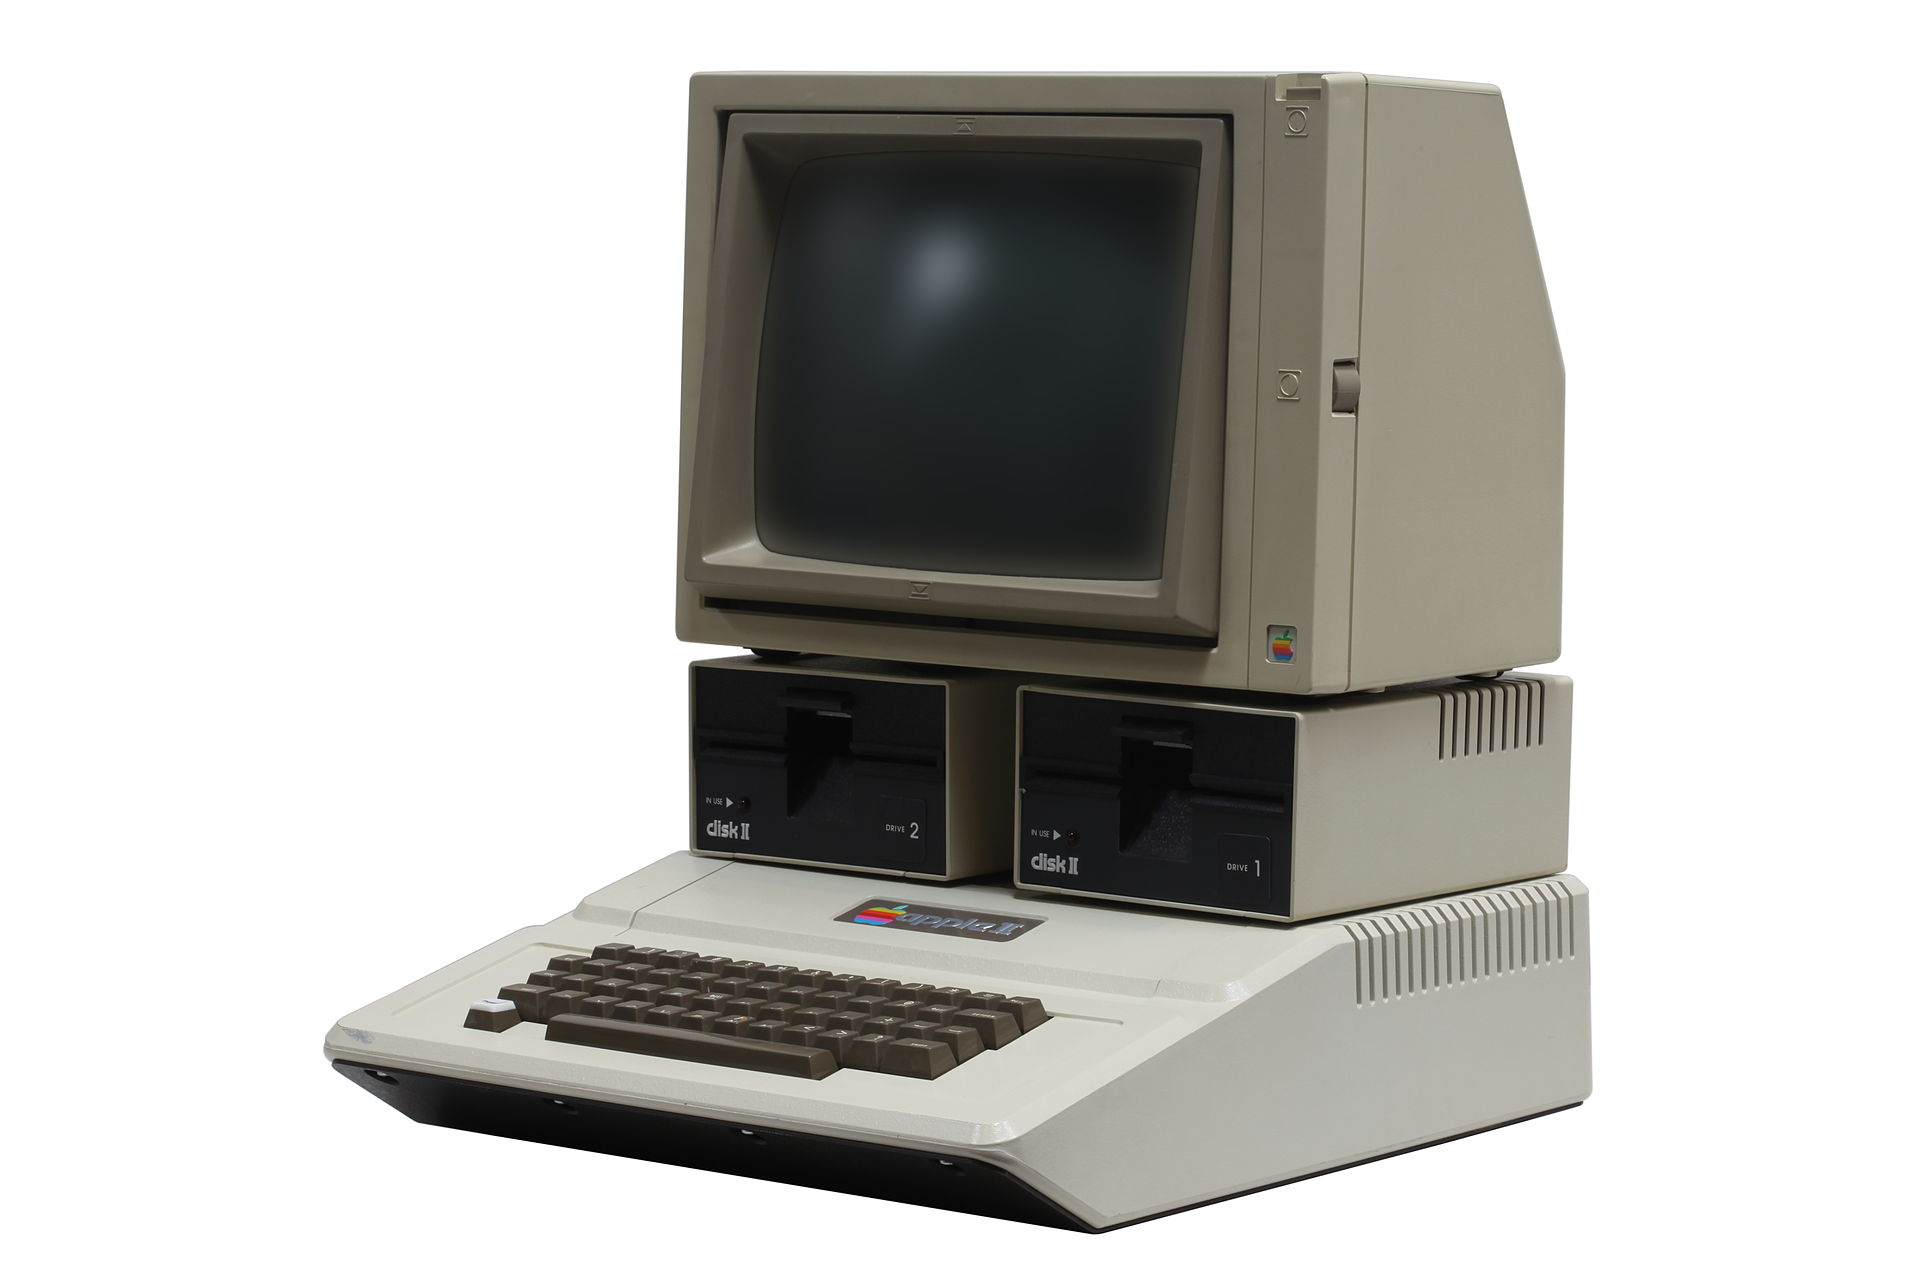
\includegraphics[scale=.05]{Media/Apple2.jpg}
    \caption{Apple II}
\end{wrapfigure}

Sorozatgyártásban a videókártya elvét elsőként 1977-ben az Apple II mikroszámítógép konstrukciójánál alkalmazták, melynek alaplapjára integrált képmegjelenítési lehetőségeit bővítőkártyák által lehetett kiegészíteni.
\end{frame}

\begin{frame}
\frametitle{Bevezetés}
\framesubtitle{Története}
\begin{wrapfigure}{r}{0.3\textwidth}
    \centering
    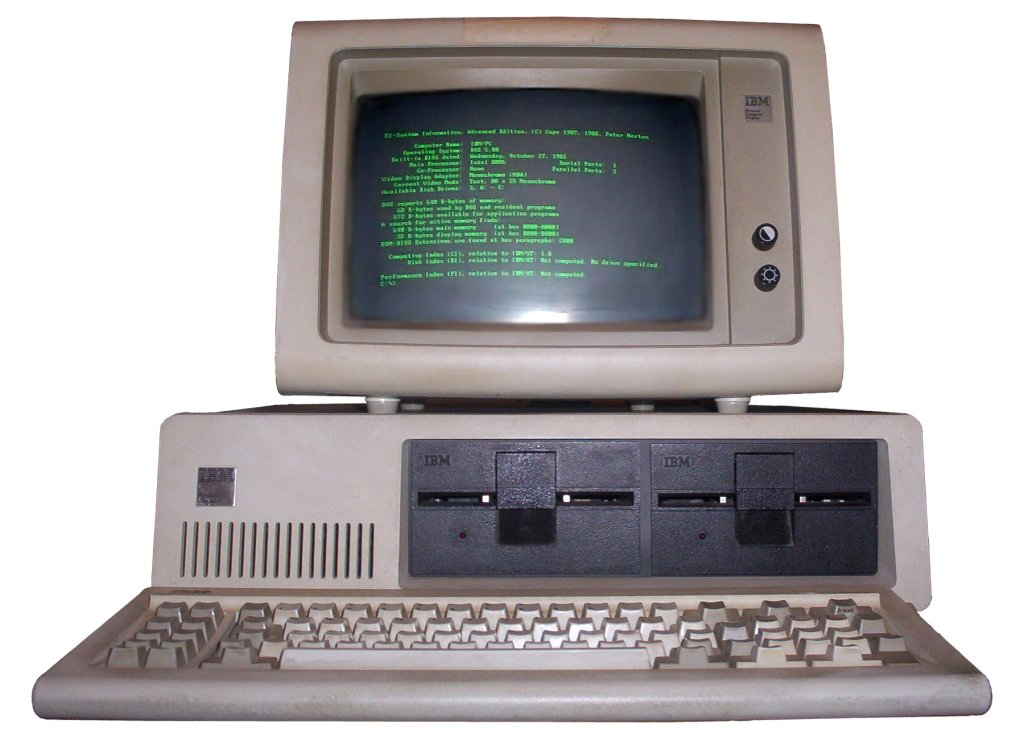
\includegraphics[scale=.09]{Media/ibmpc.jpg}
    \caption{IBM PC}
\end{wrapfigure}

Az első IBM PC 1981-ben kiadott típusában alkalmazott MDA (Monochrome Display Adapter) videókártya csupán az egyszínű, 80x25 karakteres megjelenítést tette lehetővé. Ezt követően az IBM CGA (Color Graphics Adapter) és a Hercules 1982-ben megjelent HGC (Hercules Graphics Card) videókártyái már a színes szövegkarakterek megjelenítését is támogatták.

\footnotetext[1]{\tiny https://hu.wikipedia.org/wiki/Videókártya}
\end{frame}

\subsection{GPU-k fejlődése}
\begin{frame}
\frametitle{GPU-k fejlődése}
\begin{columns}[onlytextwidth]
\begin{column}{0.5\textwidth}
\centering

\begin{figure}
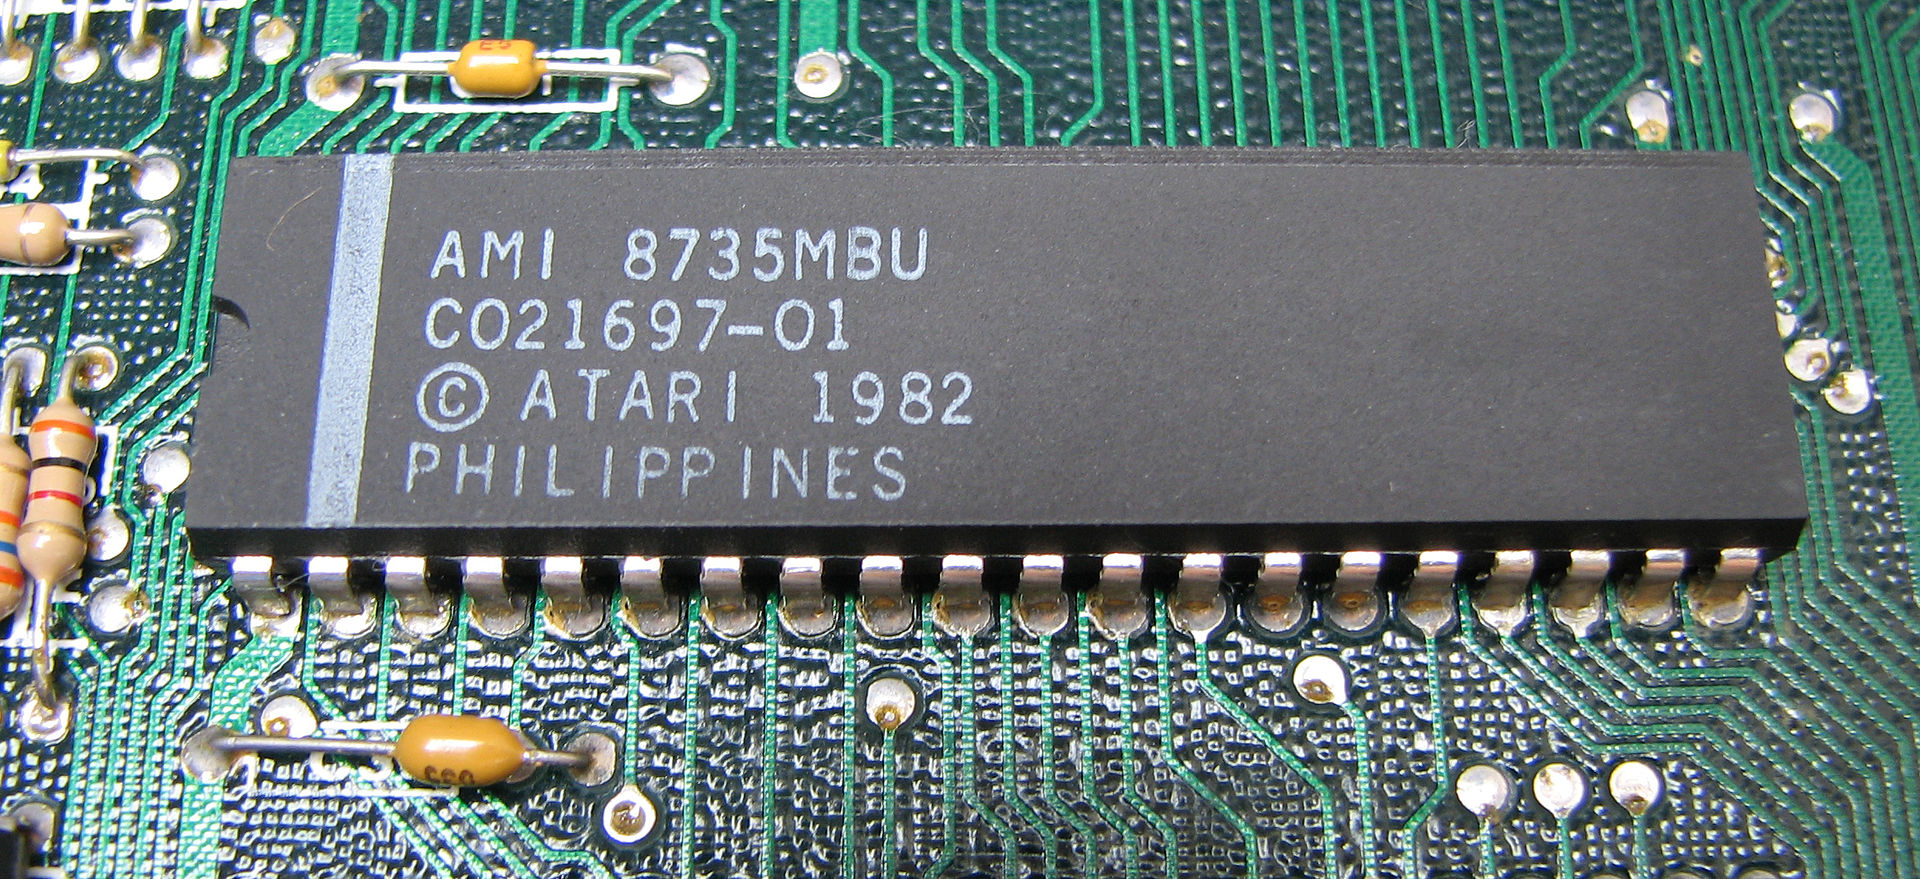
\includegraphics[scale=.12]{media/antic}
\caption{Atari ANTIC 1970-es évek}
\end{figure}

\begin{figure}
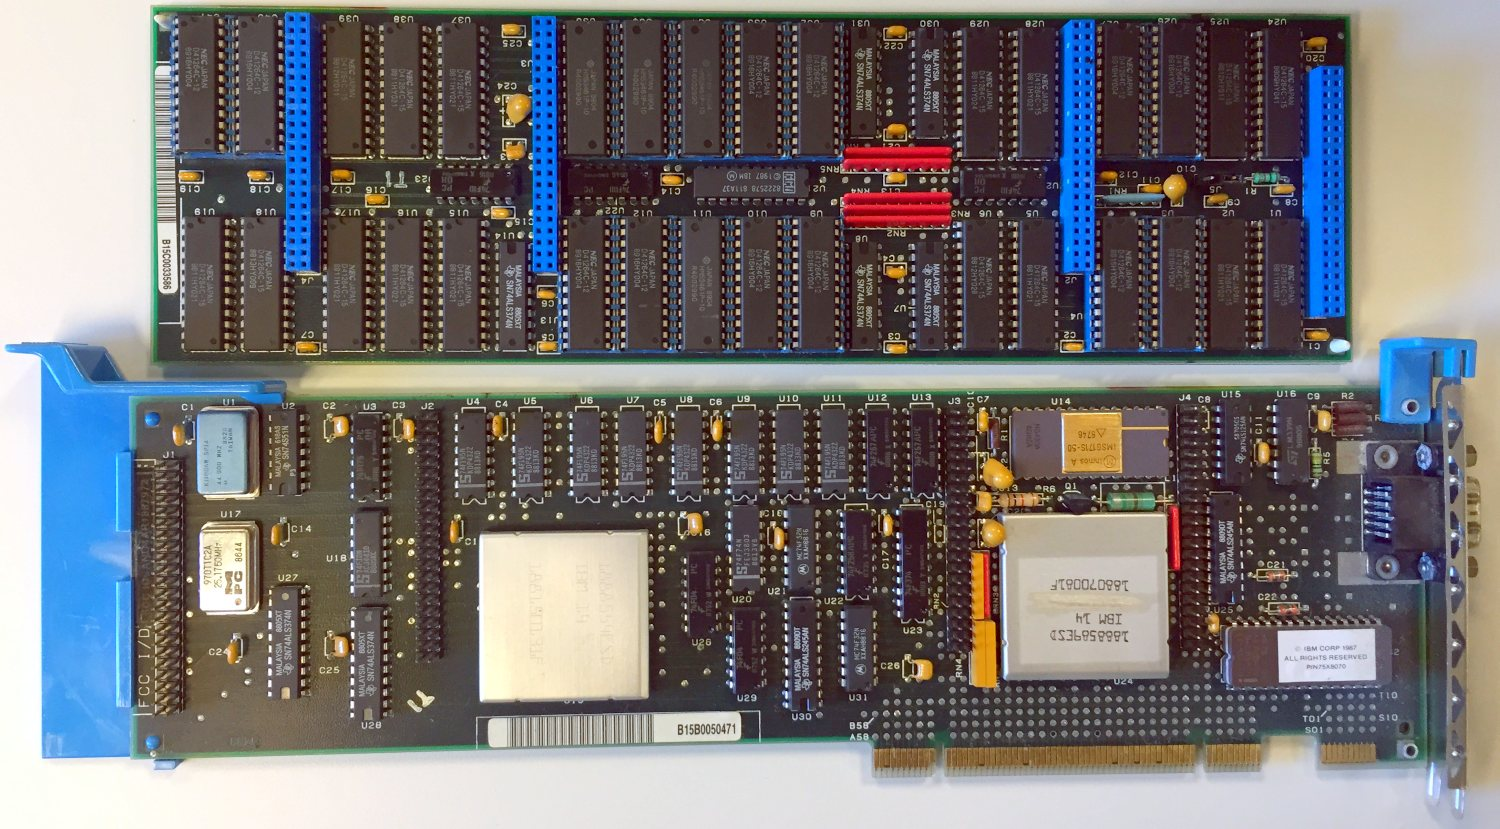
\includegraphics[scale=.07]{media/ibm}
\caption{IBM 8514 1980-as évek}
\end{figure}

\end{column}
\begin{column}{0.5\textwidth}
\centering

\begin{figure}
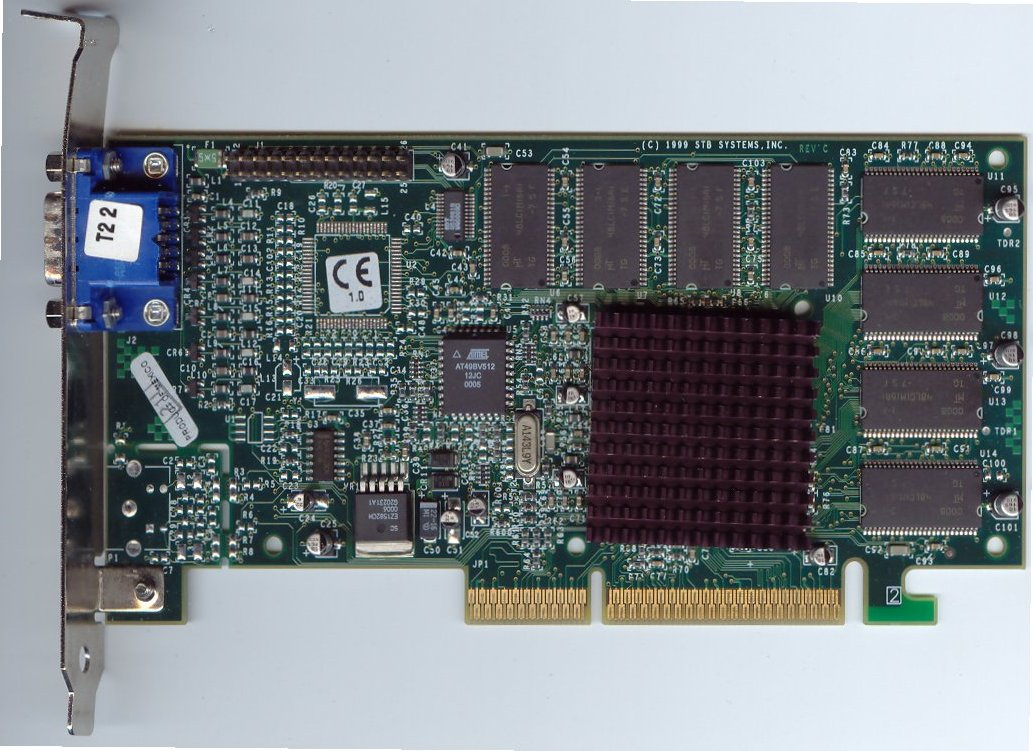
\includegraphics[scale=.15]{media/Voodoo3.jpg}
\caption{Voodoo3 1990-es évek}
\end{figure}

\begin{figure}
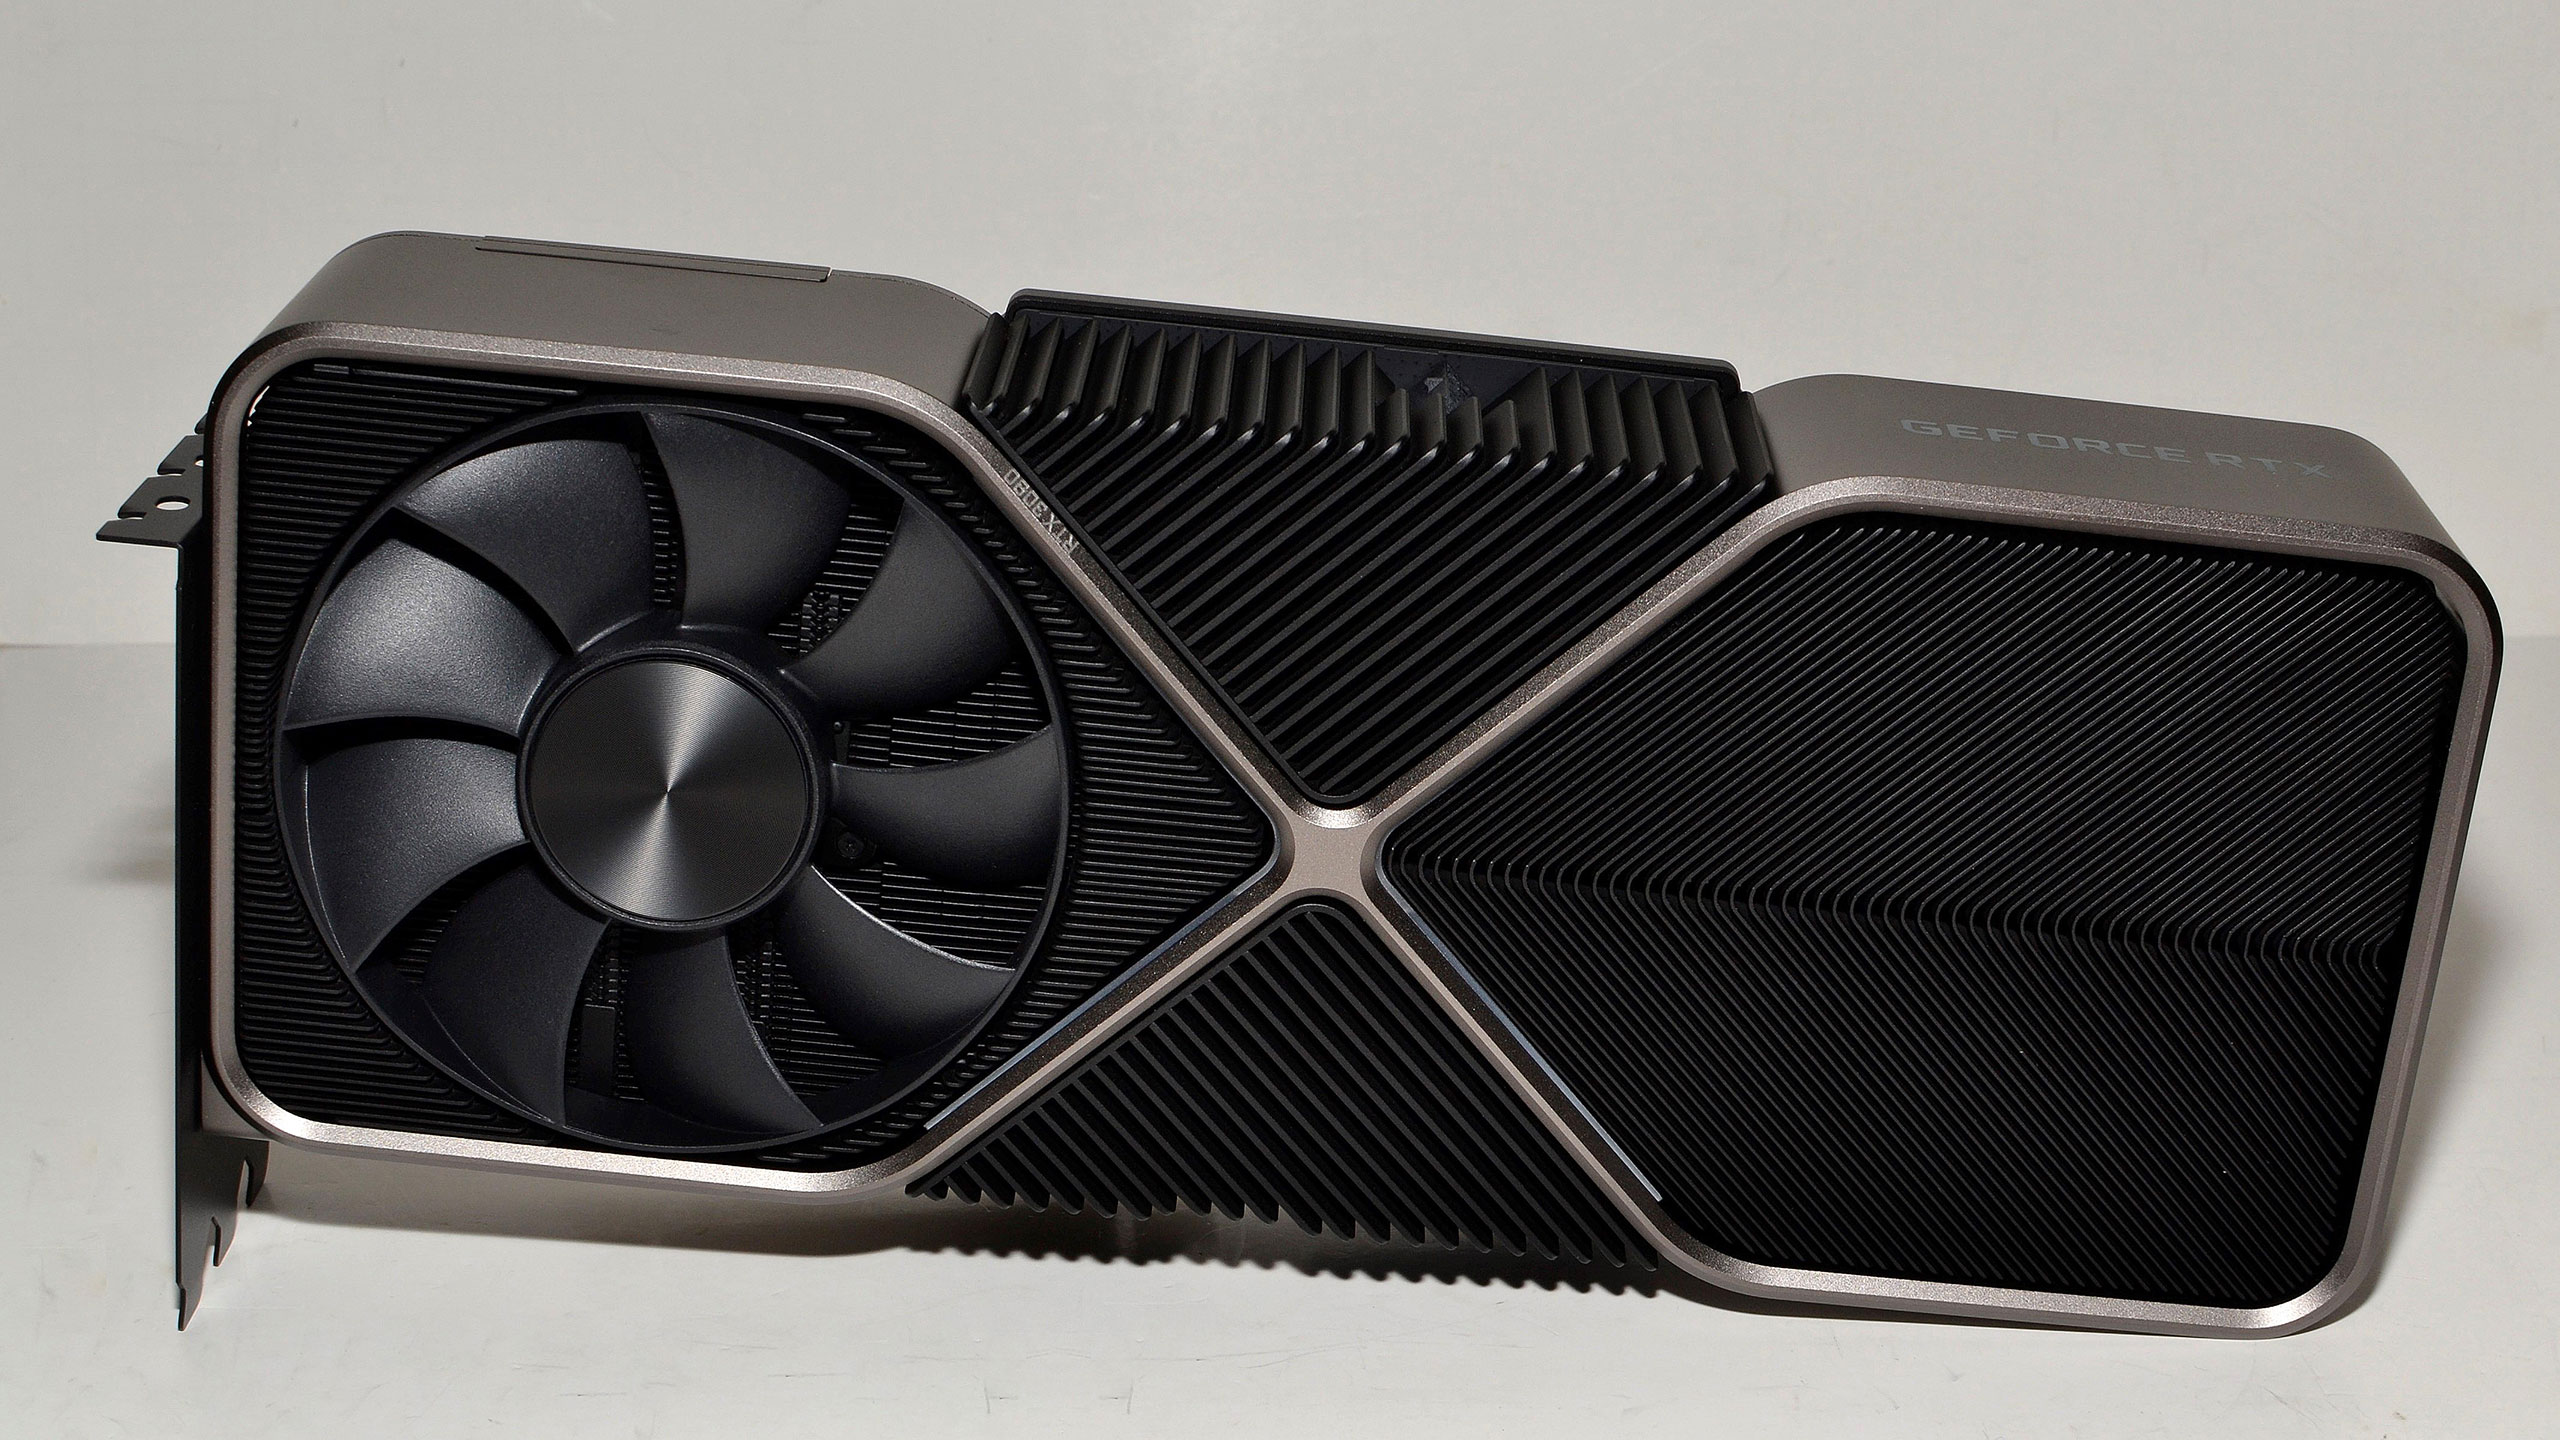
\includegraphics[scale=.035]{media/3090.jpg}
\caption{Nvidia RTX 3090 napjainkban}
\end{figure}

\end{column}
\end{columns}
\end{frame}

\section{Felépítés}
\begin{frame}
\frametitle{Vidókártyák felépítése}
\begin{figure}
\centering
\framebox{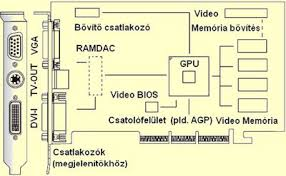
\includegraphics[scale=.5]{media/build.jpg}}
\caption{Videókártya legfontosabb részei}
\end{figure}

\end{frame}
\subsection{GPU}
\begin{frame}
\frametitle{Vidókártyák felépítése}
\framesubtitle{GPU [Graphics Processing Unit]}
A videókártya legfontosabb része, egy speciális processzor, ami grafikai műveleteket old meg 2 illetve 3 dimenzióban.\\
Feladata a grafikákat létrehozó feladatok átvétele a CPU-tól, így a processzornak nem kell grafikai számításokat végeznie, ezzel felgyorsítva a működését.\\
Hasonlóan mint a CPU a GPU is rendelkezik működési órajellel, ami a sebességét határozza meg.
\end{frame}

\subsection{Video BIOS}
\begin{frame}
\frametitle{Vidókártyák felépítése}
\framesubtitle{Video BIOS}
Minden fejlett kártya rendelkezik egy BIOS-t (\textbf{B}asic \textbf{I}nput \textbf{O}utput \textbf{S}ystem) kiegészítő Video-BIOS rendszerrel, ami biztosítja a vezérlőáramkörök sajátos képességeinek kezelését és illesztését a rendszerhez.

\end{frame}

\subsection{Video memória}
\begin{frame}
\frametitle{Vidókártyák felépítése}
\framesubtitle{Video memória}
A video memória feladata a monitoron megjelenítendő képek tárolása. A Frame-buffer a
memóriaterület azon része (akkora képpontmátrix, amekkora a képernyő felbontás),
amelybe a kiszámolt és véglegesített képpontok kerülnek. Innen jut az elkészült kép a
\textbf{RAMDAC}-on keresztül a monitorra.
\end{frame}

\subsection{Csatlakozók}
\begin{frame}
\frametitle{Vidókártyák felépítése}
\framesubtitle{Csatlakozók}

\begin{columns}[onlytextwidth]
\begin{column}{0.3\textwidth}
\begin{figure}
\centering
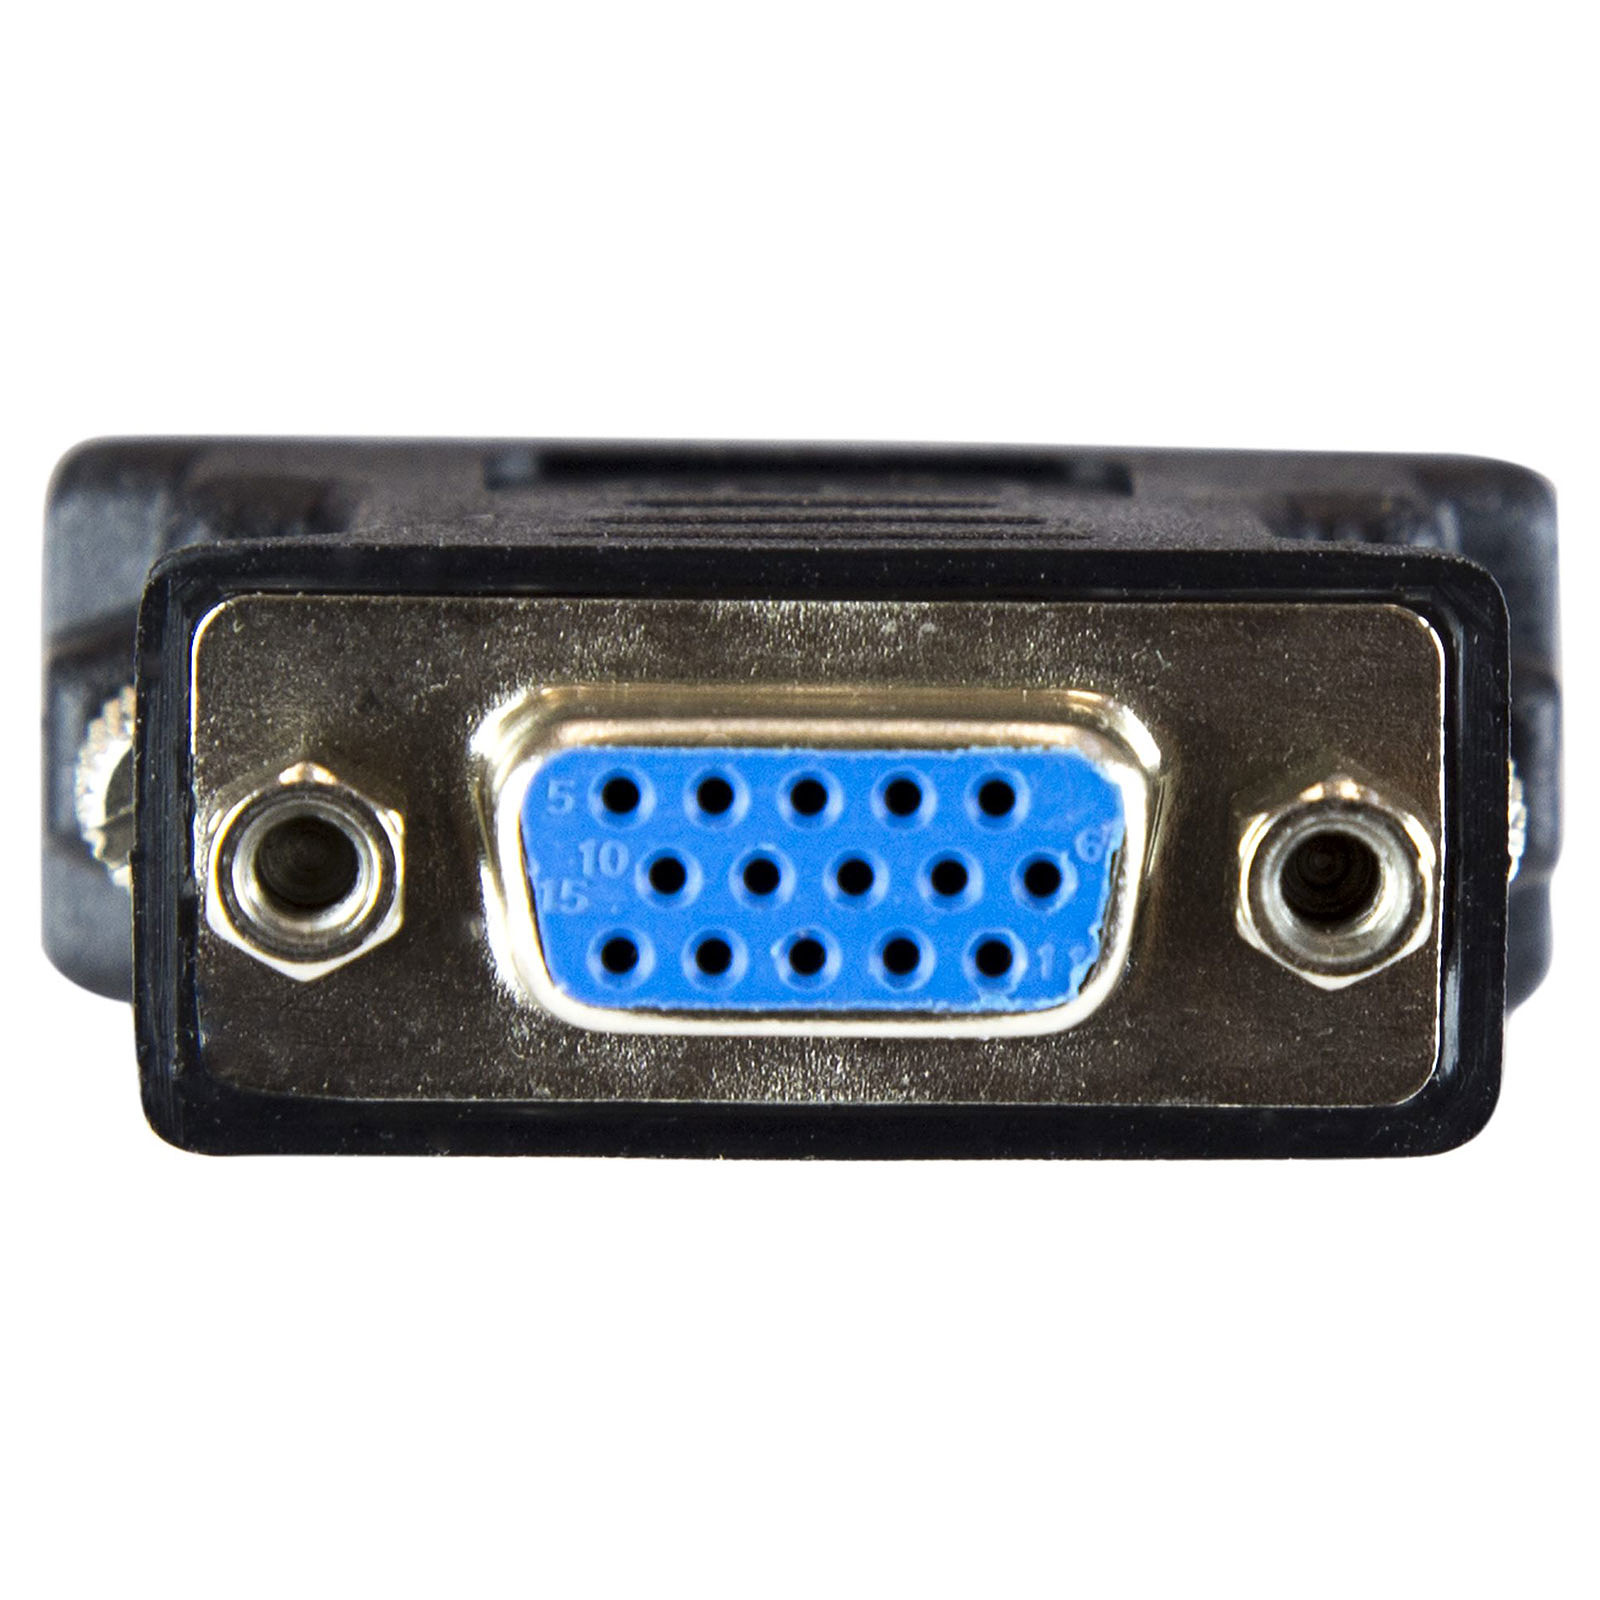
\includegraphics[scale=.045]{media/vga.jpg}
\caption{VGA}
\end{figure}
\end{column}

\begin{column}{0.3\textwidth}
\begin{figure}
\centering
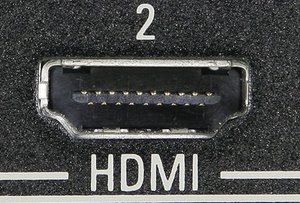
\includegraphics[scale=.25]{media/hdmi.jpg}
\caption{HDMI}
\end{figure}
\end{column}

\begin{column}{0.3\textwidth}
\begin{figure}
\centering
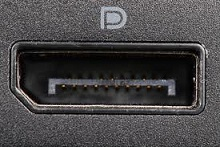
\includegraphics[scale=.3]{media/dp.jpeg}
\caption{DisplayPort}
\end{figure}
\end{column}

\end{columns}
A
videokártya ezeken keresztül biztosítja a csatlakoztatott monitor teljes működtetésével a
képernyőn történő megjelenítést.
\end{frame}

\section{Beépítés}
\begin{frame}
\frametitle{Beépítés a számítógépbe}
A mai videókártyákat a számítógép \textbf{PCI-e} (Peripheral Component Interconnect) csatlakozójába illesztve, és ha szükséges táp ellátást biztosítva tudjuk használni a gyártó által biztosított illesztőprogrammal.

\begin{figure}
\centering
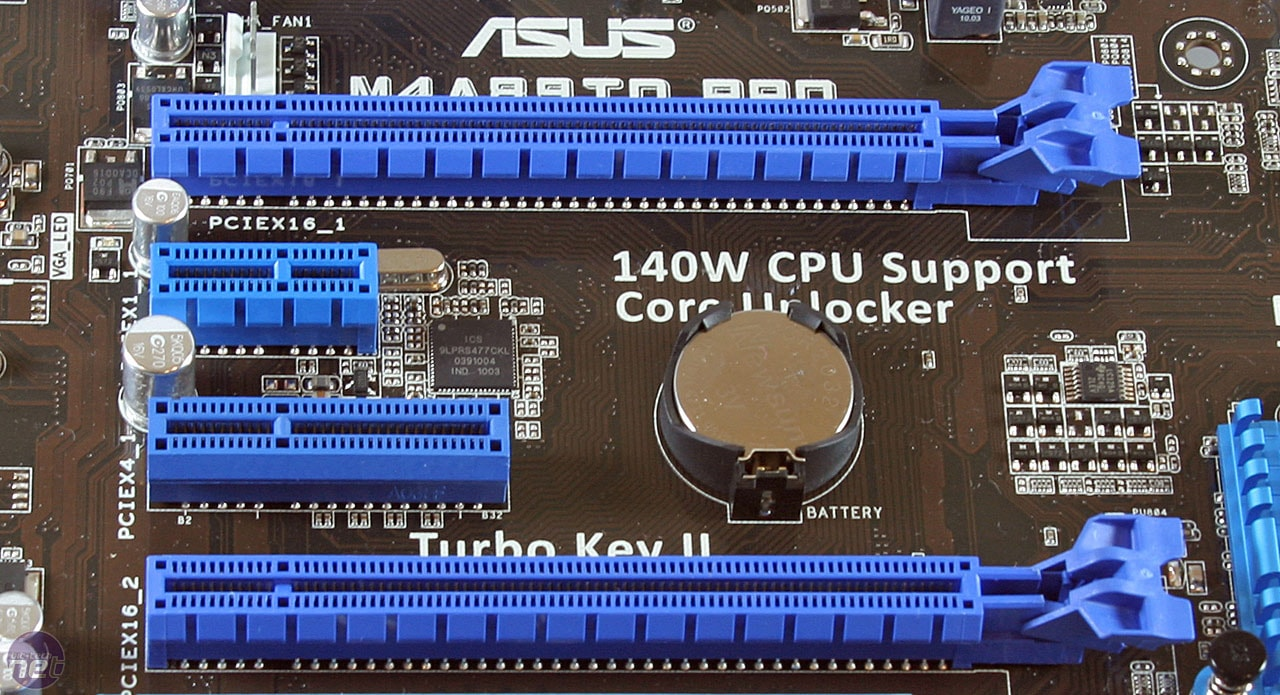
\includegraphics[scale=.09]{media/pci.jpg}
\caption{PCI-e csatlakozók}
\end{figure}
\end{frame}

\begin{frame}
\begin{center}
\begin{huge}
Köszönjük a figyelmet!
\end{huge}
\end{center}
\end{frame}
\end{document}